%% ----------------------------------------------------------------------------
%%  §8.1  Il metodo di esaustione
%% ----------------------------------------------------------------------------
\section{Il metodo di esaustione}
\label{sec:esaustione}

Con l'espressione \emph{metodo di esaustione}\index{metodo di esaustione} si indica il
procedimento con cui i matematici greci calcolavano aree e volumi di figure
curvilinee. Lo usò sistematicamente Archimede nel \textsc{iii} secolo a.C., ma, secondo
lo stesso Archimede, risale a Eudosso di Cnido (\textsc{iv} secolo a.C.). Ne abbiamo già
visto un esempio nel \cref{sec:premessa-limiti}: l'area del cerchio è stata ottenuta
come limite delle aree dei poligoni regolari inscritti, e nel \cref{teo:area-cerchio}
abbiamo dimostrato che tale limite è $\pi$. La parola «esaustione» esprime proprio
l'idea che il cerchio viene \emph{riempito}, o \emph{esaurito}, da poligoni con un
numero di lati sempre maggiore.

In questo paragrafo descriviamo il metodo con il linguaggio moderno dei limiti, su un
esempio che guiderà la definizione generale del paragrafo successivo: l'area del
\emph{settore di parabola}, cioè della regione
\begin{equation}\label{eq:settore-parabola}
  S=\set{(x,y)\in\R^{2} \tc 0\le x\le b,\ \ 0\le y\le x^{2}}, \qquad b>0,
\end{equation}
compresa tra l'asse delle $x$, il grafico di $f(x)=x^{2}$ e la retta verticale $x=b$
(\cref{fig:esaustione}, a sinistra).

\subsection{Stime per difetto e per eccesso}

Dividiamo l'intervallo $[0,b]$ in $n\in\N$ intervalli $[x_{k-1},x_{k}]$ di uguale
ampiezza $b/n$, mediante i punti
\begin{equation}\label{eq:partizione-uniforme-parabola}
  x_{0}=0,\quad x_{1}=\frac bn,\quad x_{2}=\frac{2b}n,\quad\dots,\quad
  x_{k}=\frac{kb}n,\quad\dots,\quad x_{n}=b .
\end{equation}
Poiché $f(x)=x^{2}$ è crescente in $[0,b]$, in ciascun intervallo $[x_{k-1},x_{k}]$ si
ha $x_{k-1}^{2}\le x^{2}\le x_{k}^{2}$. Il rettangolo di base $[x_{k-1},x_{k}]$ e altezza
$x_{k-1}^{2}$ è dunque contenuto in $S$, mentre quello di uguale base e altezza
$x_{k}^{2}$ contiene la parte di $S$ che sta sopra $[x_{k-1},x_{k}]$
(\cref{fig:esaustione}, al centro e a destra). Sommando le aree dei rettangoli
otteniamo
\begin{align}
  s_{n}&=\sum_{k=1}^{n}f(x_{k-1})(x_{k}-x_{k-1})=\frac bn\sum_{k=1}^{n}x_{k-1}^{2}
  =\frac bn\bigl(x_{0}^{2}+x_{1}^{2}+\dots+x_{n-1}^{2}\bigr),
  \label{eq:somma-inferiore-parabola}\\
  S_{n}&=\sum_{k=1}^{n}f(x_{k})(x_{k}-x_{k-1})=\frac bn\sum_{k=1}^{n}x_{k}^{2}
  =\frac bn\bigl(x_{1}^{2}+x_{2}^{2}+\dots+x_{n}^{2}\bigr).
  \label{eq:somma-superiore-parabola}
\end{align}
La prima è l'area di un'unione di rettangoli (un \emph{plurirettangolo}) contenuta in
$S$, la seconda quella di un plurirettangolo che contiene $S$. Se attribuiamo all'area
le proprietà che l'intuizione suggerisce (l'area di un rettangolo è base per altezza,
l'area di un'unione di figure senza punti interni comuni è la somma delle aree, una
figura contenuta in un'altra ha area minore o uguale), otteniamo
\begin{equation}\label{eq:stime-parabola}
  s_{n}\le\text{area }S\le S_{n} \qquad\perogni n\in\N .
\end{equation}
La somma $s_{n}$ è detta \emph{somma integrale inferiore}, la somma $S_{n}$
\emph{somma integrale superiore}.

\begin{figure}[htb]
\centering
\begin{tikzpicture}
\begin{axis}[name=p1, width=0.38\textwidth, height=0.36\textwidth,
  axis lines=left, xmin=0, xmax=1.15, ymin=0, ymax=1.15, xtick={1},
  xticklabels={$b$}, ytick={1}, yticklabels={$b^{2}$},
  title={\scriptsize il settore $S$}, clip=false]
  \addplot[draw=none, fill=blu!18, domain=0:1, samples=60] {x^2} \closedcycle;
  \addplot[curva, domain=0:1.08, samples=60] {x^2};
  \addplot[tratteggio] coordinates {(1,0) (1,1)};
  \node[font=\scriptsize, blu] at (axis cs:0.72,0.2) {$S$};
  \node[font=\scriptsize, anchor=east] at (axis cs:0.95,0.95) {$y=x^{2}$};
\end{axis}
\begin{axis}[at={(p1.east)}, anchor=west, xshift=0.5cm, name=p2,
  width=0.38\textwidth, height=0.36\textwidth, axis lines=left, xmin=0, xmax=1.15,
  ymin=0, ymax=1.15, xtick={0,0.1667,0.3333,0.5,0.6667,0.8333,1},
  xticklabels={,,,,,,$b$}, ytick=\empty, title={\scriptsize $s_{6}$ (per difetto)}]
  \addplot[ybar interval, fill=blu!25, draw=blu, domain=0:1, samples=7] {x^2};
  \addplot[curva2, domain=0:1.08, samples=60] {x^2};
\end{axis}
\begin{axis}[at={(p2.east)}, anchor=west, xshift=0.5cm, width=0.38\textwidth,
  height=0.36\textwidth, axis lines=left, xmin=0, xmax=1.15, ymin=0, ymax=1.15,
  xtick={0,0.1667,0.3333,0.5,0.6667,0.8333,1}, xticklabels={,,,,,,$b$},
  ytick=\empty, title={\scriptsize $S_{6}$ (per eccesso)}]
  \addplot[ybar interval, fill=rame!25, draw=rame, domain=0:1, samples=7]
    {(x+1/6)^2};
  \addplot[curva, domain=0:1.08, samples=60] {x^2};
\end{axis}
\end{tikzpicture}
\caption{Il settore di parabola $S$ (a sinistra) e le sue approssimazioni con $n=6$
rettangoli: per difetto, con altezze $x_{k-1}^{2}$ (al centro), e per eccesso, con
altezze $x_{k}^{2}$ (a destra).}
\label{fig:esaustione}
\end{figure}

Calcoliamo le due somme. Ricordando che $x_{k}=kb/n$ e usando la formula della somma
dei primi $n$ quadrati, dimostrata per induzione nella \cref{prop:quadrati},
\[
  \sum_{k=1}^{n}x_{k}^{2}=\frac{b^{2}}{n^{2}}\sum_{k=1}^{n}k^{2}
  =\frac{b^{2}}{n^{2}}\cdot\frac{n(n+1)(2n+1)}6 ,
\]
e quindi $S_{n}=\frac bn\sum x_{k}^{2}$ vale
\begin{equation}\label{eq:Sn-parabola}
  S_{n}=\frac{b^{3}}6\cdot\frac{(n+1)(2n+1)}{n^{2}} .
\end{equation}
Nella somma inferiore compaiono i quadrati di $x_{0},\dots,x_{n-1}$, cioè la stessa somma
con $n-1$ al posto di $n$ (il termine $x_{0}^{2}=0$ non contribuisce):
\begin{equation}\label{eq:sn-parabola}
  s_{n}=\frac bn\cdot\frac{b^{2}}{n^{2}}\cdot\frac{(n-1)n(2n-1)}6
  =\frac{b^{3}}6\cdot\frac{(n-1)(2n-1)}{n^{2}} .
\end{equation}
Prima di passare al limite osserviamo una semplificazione notevole. La differenza tra
le due somme è una somma \emph{telescopica}, nella quale i termini intermedi si
cancellano a due a due (come nella \cref{prop:telescopica}):
\begin{equation}\label{eq:differenza-parabola}
  S_{n}-s_{n}=\frac bn\sum_{k=1}^{n}\bigl(x_{k}^{2}-x_{k-1}^{2}\bigr)
  =\frac bn\bigl(x_{n}^{2}-x_{0}^{2}\bigr)=\frac{b^{3}}n .
\end{equation}
Il significato geometrico è illuminante: i rettangolini di base $[x_{k-1},x_{k}]$ e
altezza $x_{k}^{2}-x_{k-1}^{2}$, che costituiscono la differenza tra i due
plurirettangoli, traslati orizzontalmente fino all'ultima colonna vi si impilano senza
sovrapporsi,
formando un unico rettangolo di base $b/n$ e altezza $b^{2}$ (\cref{fig:telescopica}).
La differenza tende a zero come $1/n$.

\begin{figure}[htb]
\centering
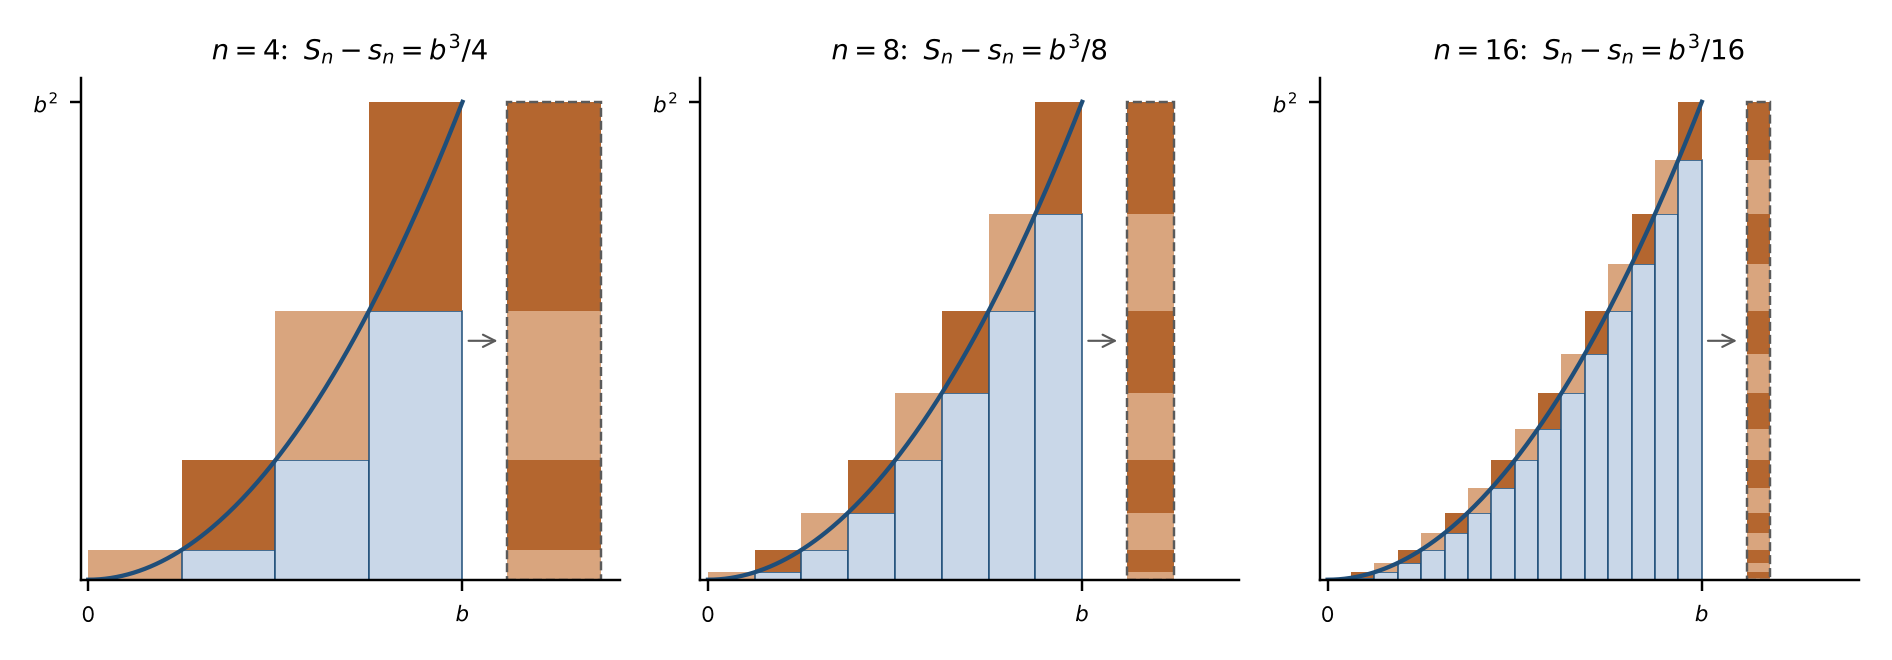
\includegraphics[width=\textwidth]{figure/esaustione.png}
\caption{La differenza $S_{n}-s_{n}=b^{3}/n$ per $n=4,8,16$. I rettangolini in color rame
(la parte di plurirettangolo circoscritto che eccede quello inscritto) si possono
traslare nell'ultima colonna, dove formano il rettangolo tratteggiato di base $b/n$ e
altezza $b^{2}$: la differenza vale esattamente $b^{3}/n$
(\texttt{python/fig\_esaustione.py}).}
\label{fig:telescopica}
\end{figure}

\needspace{12\baselineskip}
\subsection{L'area del settore di parabola}

\begin{proposizione}[Area del settore di parabola]\label{prop:settore-parabola}
Sia $b>0$ e siano $s_{n}$, $S_{n}$ le somme
\eqref{eq:somma-inferiore-parabola}--\eqref{eq:somma-superiore-parabola}. Allora
$b^{3}/3$ è l'\emph{unico} numero reale $c$ tale che
\begin{equation}\label{eq:separatore-parabola}
  s_{n}\le c\le S_{n} \qquad\perogni n\in\N .
\end{equation}
\end{proposizione}

\begin{schema}
\Ipotesi{$b>0$; \ $s_{n}$, $S_{n}$ somme inferiori e superiori di $x^{2}$ in $[0,b]$
relative alla suddivisione in $n$ parti uguali.}
\Tesi{(i) $s_{n}<\frac{b^{3}}3<S_{n}$ per ogni $n$; \ (ii) se $s_{n}\le c\le S_{n}$ per ogni
$n$, allora $c=\frac{b^{3}}3$.}
\end{schema}

\begin{strategia}
Le formule \eqref{eq:Sn-parabola} e \eqref{eq:sn-parabola} sono esplicite: sviluppando i
prodotti, entrambe si scrivono come $\frac{b^{3}}3$ più o meno termini che contengono
$\frac1n$ e $\frac1{n^{2}}$, e un confronto di segni prova la (i). Per l'unicità basta
osservare che due numeri compresi tra $s_{n}$ e $S_{n}$ distano al più
$S_{n}-s_{n}=\frac{b^{3}}n$, quantità che, per la proprietà di Archimede, diventa più
piccola di qualsiasi numero positivo assegnato.
\end{strategia}

\begin{dimostrazione}
(i) Sviluppando i prodotti nelle \eqref{eq:Sn-parabola} e \eqref{eq:sn-parabola},
\[
\begin{aligned}
  S_{n}&=\frac{b^{3}}6\cdot\frac{2n^{2}+3n+1}{n^{2}}
  =\frac{b^{3}}3+\frac{b^{3}}{2n}+\frac{b^{3}}{6n^{2}},\\
  s_{n}&=\frac{b^{3}}6\cdot\frac{2n^{2}-3n+1}{n^{2}}
  =\frac{b^{3}}3-\frac{b^{3}}{6n^{2}}\,(3n-1) .
\end{aligned}
\]
La prima mostra che $S_{n}>\frac{b^{3}}3$; nella seconda $3n-1>0$ per ogni $n\ge1$, e
quindi $s_{n}<\frac{b^{3}}3$.

(ii) Sia $c$ un numero che verifica la \eqref{eq:separatore-parabola}. Poiché anche
$\frac{b^{3}}3$ la verifica, i due numeri appartengono entrambi all'intervallo
$[s_{n},S_{n}]$, e quindi, per la \eqref{eq:differenza-parabola},
\[
  \Bigl|c-\frac{b^{3}}3\Bigr|\le S_{n}-s_{n}=\frac{b^{3}}n \qquad\perogni n\in\N .
\]
Se fosse $c\neq\frac{b^{3}}3$, per la proprietà di Archimede (\cref{teo:archimede})
esisterebbe $n\in\N$ con $n\,\bigl|c-\frac{b^{3}}3\bigr|>b^{3}$, contro la disuguaglianza
appena scritta. Dunque $c=\frac{b^{3}}3$.
\end{dimostrazione}

Dalle \eqref{eq:stime-parabola} e dalla proposizione segue che, se il settore $S$ ha
un'area, essa non può che essere
\begin{equation}\label{eq:area-parabola}
  \text{area }S=\frac{b^{3}}3 ,
\end{equation}
cioè \emph{un terzo} dell'area del rettangolo $[0,b]\times[0,b^{2}]$ che lo contiene.
È il risultato di Archimede. Allo stesso valore si arriva passando al limite nelle
\eqref{eq:Sn-parabola}--\eqref{eq:sn-parabola} (basta dividere numeratore e denominatore
per $n^{2}$): $s_{n}\to\frac{b^{3}}3$ e $S_{n}\to\frac{b^{3}}3$. Le due strade sono
equivalenti, ma la prima, che caratterizza l'area come \emph{unico elemento separatore}
tra le stime per difetto e quelle per eccesso, è quella che generalizzeremo.

Il programma seguente calcola le somme in aritmetica razionale esatta, con il modulo
\texttt{fractions}, per $b=1$: si vede la differenza $S_{n}-s_{n}=\frac1n$ e
l'avvicinamento di entrambe le somme a $\frac13$.

\begin{python}[Somme integrali del settore di parabola in aritmetica esatta]
from fractions import Fraction as F

def somme(n, b=F(1)):
    """Somme inferiore e superiore di x^2 in [0, b], n intervalli."""
    x = [F(k, n) * b for k in range(n + 1)]
    s = sum(x[k - 1]**2 * (x[k] - x[k - 1]) for k in range(1, n + 1))
    S = sum(x[k]**2 * (x[k] - x[k - 1]) for k in range(1, n + 1))
    return s, S

print(f"{'n':>5} {'s_n':>10} {'S_n':>10} {'S_n - s_n':>10}")
for n in (1, 2, 5, 10, 100, 1000):
    s, S = somme(n)
    print(f"{n:5d} {float(s):10.6f} {float(S):10.6f}"
          f" {float(S - s):10.6f}")
s, S = somme(10)
print("n = 10, valori esatti:", s, "< 1/3 <", S)
\end{python}
\begin{risultato}
    n        s_n        S_n  S_n - s_n
    1   0.000000   1.000000   1.000000
    2   0.125000   0.625000   0.500000
    5   0.240000   0.440000   0.200000
   10   0.285000   0.385000   0.100000
  100   0.328350   0.338350   0.010000
 1000   0.332834   0.333834   0.001000
n = 10, valori esatti: 57/200 < 1/3 < 77/200
\end{risultato}

\begin{osservazione}[Un indizio del teorema fondamentale]\label{oss:indizio-tfc}
Pensiamo l'area \eqref{eq:area-parabola} come funzione dell'estremo $b$ e deriviamola:
\begin{equation}\label{eq:derivata-area}
  \frac{d}{db}\Bigl(\frac{b^{3}}3\Bigr)=b^{2} .
\end{equation}
La derivata dell'area è il valore in $x=b$ della funzione $f(x)=x^{2}$ che delimita la
regione. Non è una coincidenza: se si sposta l'estremo da $b$ a $b+h$, l'area aumenta
di una striscia di base $h$ e altezza circa $b^{2}$, e il rapporto incrementale è
circa $b^{2}$. Questa osservazione, resa rigorosa, è il \emph{teorema fondamentale del
calcolo integrale}, che dimostreremo nel prossimo capitolo e che trasformerà il
calcolo delle aree in un problema di derivate.
\end{osservazione}

\begin{idea}[La teoria delle strisce e la portanza di un'ala]
Lungo l'apertura alare la portanza non è distribuita uniformemente: si descrive con la
\emph{portanza per unità di apertura} $l(y)$, misurata in N/m, dove $y\in[-\frac b2,
\frac b2]$ è la coordinata lungo l'apertura $b$. La portanza totale è l'«area» sotto il
grafico di $l$: per calcolarla, la \emph{teoria delle strisce} divide l'ala in strisce
di larghezza $\Delta y$ e somma i contributi $l(y_{k})\,\Delta y$, esattamente come
abbiamo fatto per la parabola. Un caso fondamentale è la \emph{distribuzione
ellittica}
\begin{equation}\label{eq:portanza-ellittica}
  l(y)=l_{0}\sqrt{1-\Bigl(\frac{2y}b\Bigr)^{2}}, \qquad -\frac b2\le y\le\frac b2,
\end{equation}
che, secondo la teoria della linea portante di Ludwig Prandtl (1918), rende minima la
resistenza indotta a parità di portanza e di apertura; la si ottiene, ad esempio, con
un'ala di pianta ellittica come quella dello Spitfire (\cref{fig:portanza-ellittica}).
Poiché $l$ è crescente in $[-\frac b2,0]$ e decrescente in $[0,\frac b2]$, se lo zero è
un estremo delle strisce, in ogni striscia il minimo e il massimo di $l$ sono assunti
negli estremi della striscia, e le somme per difetto e per eccesso si calcolano
facilmente. Vedremo nell'\cref{es:portanza-ellittica-esatta} che l'area sotto la
\eqref{eq:portanza-ellittica} vale $\frac\pi4l_{0}b$; per un velivolo di peso
$W=10\,000$~N e apertura $b=10$~m, il volo livellato ($L=W$) richiede dunque
$l_{0}=\frac{4W}{\pi b}\approx1273$~N/m.
\end{idea}

\begin{python}[Portanza totale con la teoria delle strisce]
import math

b, W = 10.0, 10000.0                  # apertura [m], peso [N]
l0 = 4 * W / (math.pi * b)            # carico al centro [N/m]

def l(y):
    """Portanza per unità di apertura, distribuzione ellittica."""
    return l0 * math.sqrt(max(0.0, 1 - (2 * y / b)**2))

def strisce(n):
    """Somme per difetto e per eccesso con n strisce (n pari)."""
    y = [-b / 2 + k * b / n for k in range(n + 1)]
    s = S = 0.0
    for k in range(1, n + 1):
        lo, hi = sorted((l(y[k - 1]), l(y[k])))  # l monotona
        s += lo * (y[k] - y[k - 1])
        S += hi * (y[k] - y[k - 1])
    return s, S

print(f"l0 = {l0:.2f} N/m")
for n in (4, 16, 64, 256, 1024):
    s, S = strisce(n)
    print(f"n = {n:4d}: {s:8.1f} N <= L <= {S:8.1f} N"
          f"   (S - s = {S - s:6.1f} N)")
\end{python}
\begin{risultato}
l0 = 1273.24 N/m
n =    4:   5513.3 N <= L <=  11879.5 N   (S - s = 6366.2 N)
n =   16:   9039.4 N <= L <=  10631.0 N   (S - s = 1591.5 N)
n =   64:   9780.4 N <= L <=  10178.3 N   (S - s =  397.9 N)
n =  256:   9947.7 N <= L <=  10047.2 N   (S - s =   99.5 N)
n = 1024:   9987.2 N <= L <=  10012.1 N   (S - s =   24.9 N)
\end{risultato}

\begin{figure}[htb]
\centering
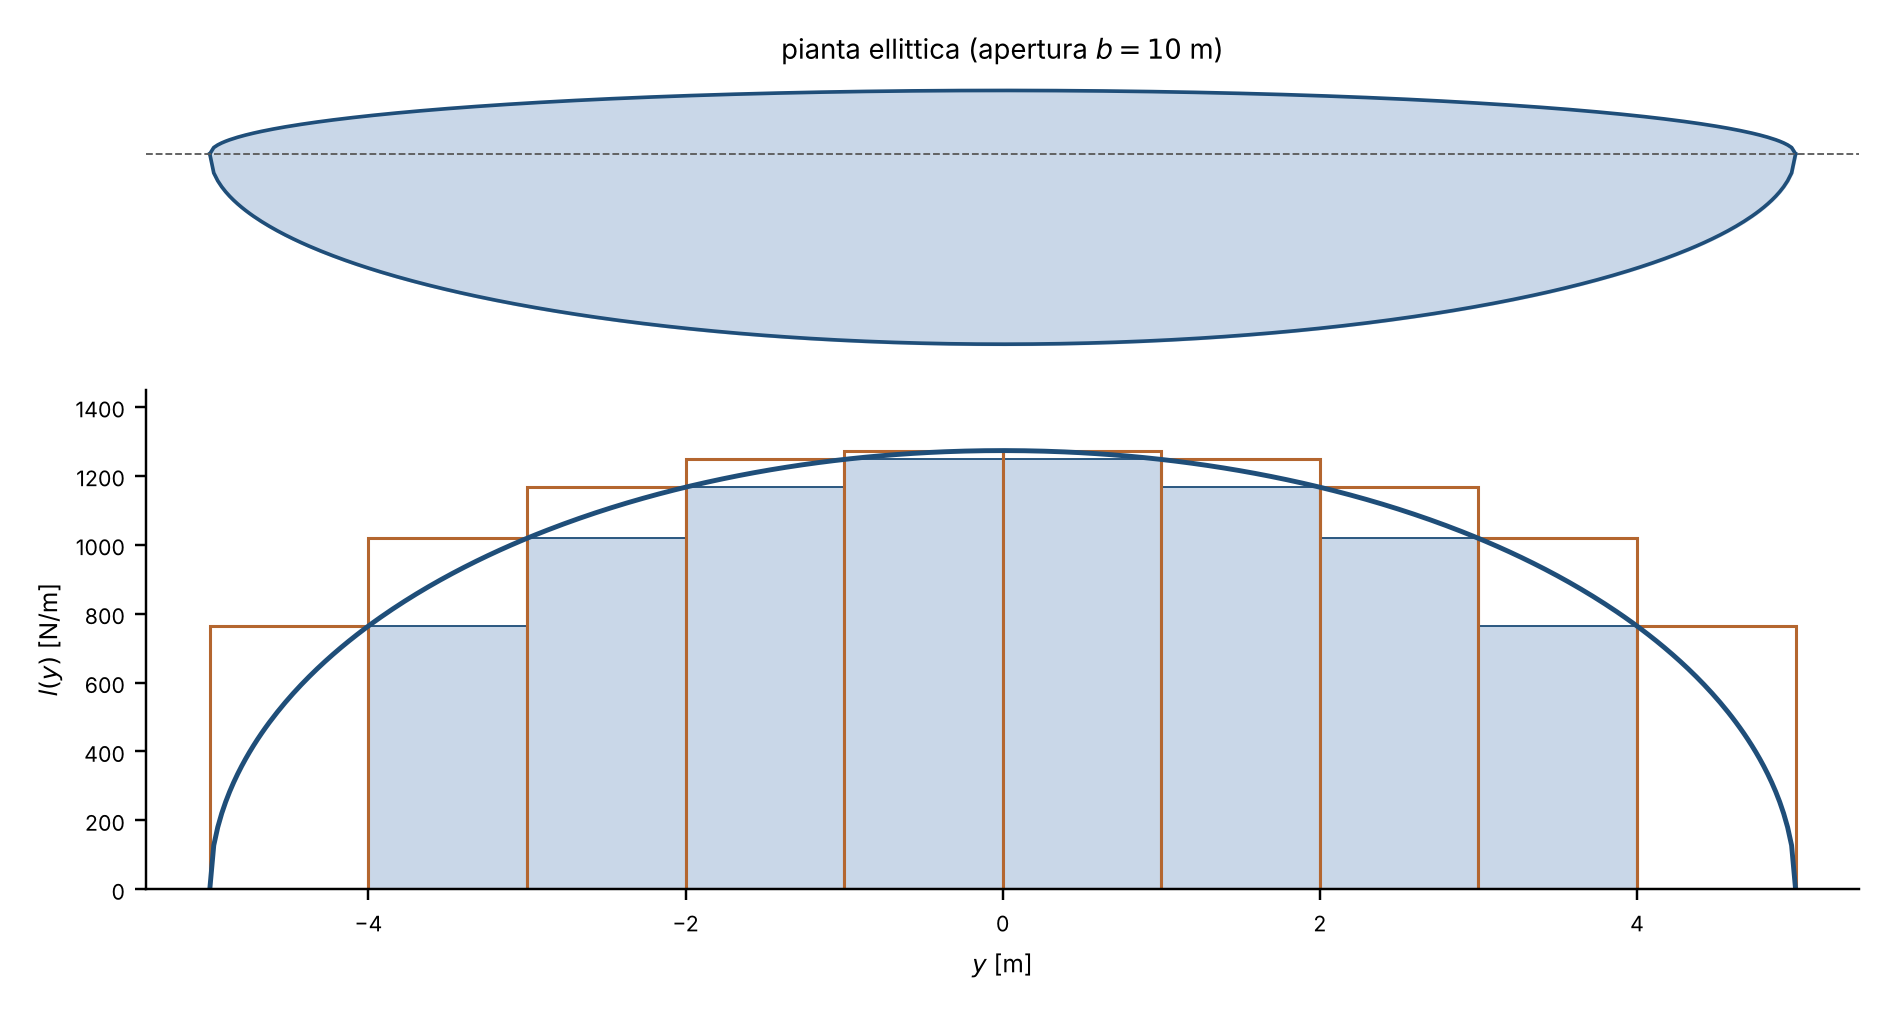
\includegraphics[width=\textwidth]{figure/portanza_ellittica.png}
\caption{In alto, la pianta ellittica di un'ala di apertura $b=10$~m. In basso, la
distribuzione ellittica della portanza \eqref{eq:portanza-ellittica} con $10$ strisce:
in azzurro i rettangoli della somma per difetto, in color rame il contorno di quelli
della somma per eccesso (\texttt{python/fig\_portanza\_ellittica.py}).}
\label{fig:portanza-ellittica}
\end{figure}

Anche qui la differenza tra le due somme è telescopica: in ciascuna delle due metà
dell'ala, dove $l$ è monotòna e passa dal valore $0$ al valore $l_{0}$, essa vale
$\frac{l_{0}b}n$, e in totale $S-s=\frac{2l_{0}b}n$. Le somme convergono al valore
esatto $10\,000$~N, ma lentamente, come $1/n$: nel \cref{sec:integrabilita-continue}
vedremo formule di approssimazione molto più efficienti.

\begin{notastorica}[Da Eudosso a Fermat]
Eudosso di Cnido (circa 408--355 a.C.) è considerato l'inventore del metodo di
esaustione, con il quale dimostrò, ad esempio, che il volume di un cono è un terzo di
quello del cilindro con la stessa base e la stessa altezza. Archimede di Siracusa
(circa 287--212 a.C.) ne fece uno strumento potentissimo: nella \emph{Quadratura della
parabola} dimostrò che il segmento parabolico ha un'area uguale ai $\frac43$ di quella
del triangolo inscritto con la stessa base e lo stesso vertice (ne seguiremo il
ragionamento nel \S\ref{subsec:archimede-parabola}). L'esaustione restò per due
millenni il modello del rigore, ma andava reinventata per ogni figura; nel Seicento si
cercarono scorciatoie. Keplero, nella \emph{Nova stereometria doliorum vinariorum}
(1615), vide il cerchio come formato da infiniti triangolini con il vertice nel centro.
Bonaventura Cavalieri, allievo di Galileo, nella \emph{Geometria indivisibilibus
continuorum} (1635) trattò le figure piane come insiemi di infinite corde parallele, gli
\emph{indivisibili}, e ne ricavò il \emph{principio di Cavalieri}: due figure tagliate da
ogni parallela a una retta data secondo corde uguali hanno la stessa area. Evangelista
Torricelli, nell'\emph{Opera geometrica} (1644), diede una ventina di dimostrazioni del
teorema di Archimede, alcune alla maniera degli antichi, altre con gli indivisibili.
John Wallis, nell'\emph{Arithmetica infinitorum} (1656), osservò che il rapporto tra
$0^{2}+1^{2}+\dots+n^{2}$ e $(n+1)\,n^{2}$ vale $\frac13+\frac1{6n}$, e ne concluse che
«all'infinito» esso diventa $\frac13$: è la \eqref{eq:area-parabola}. Pierre de Fermat,
negli stessi anni, calcolò l'area sotto le curve $y=x^{n}$ suddividendo l'intervallo
con punti in progressione geometrica. Questi metodi guadagnavano in generalità ciò che perdevano in rigore; le
somme integrali di questo capitolo conservano l'una e l'altro.
\end{notastorica}

\subsection{Approfondimento: la quadratura della parabola di Archimede}
\label{subsec:archimede-parabola}

Archimede non usò rettangoli, ma «esaurì» il segmento di parabola con triangoli:
inscrisse nel segmento un triangolo, nei due segmenti rimasti scoperti altri due
triangoli, e così via. Seguiamo il suo ragionamento sulla parabola $y=x^{2}$, con le
coordinate, che Archimede non aveva. Come nel \cref{sec:esaustione}, attribuiamo
all'area le proprietà suggerite dall'intuizione (aree elementari, additività per figure
senza punti interni comuni, confronto per inclusione); non useremo né limiti né serie,
ma soltanto una somma finita e la proprietà di Archimede.

Siano $p<r$ e siano $A=(p,p^{2})$, $B=(r,r^{2})$ due punti della parabola. La retta
$AB$ ha equazione $y=c(x)$, con $c(x)=(p+r)x-pr$, come si verifica sostituendo $x=p$ e
$x=r$. Chiamiamo \emph{segmento parabolico} di corda $AB$ la regione
\begin{equation}\label{eq:segmento-parabolico}
  \Sigma(p,r)=\set{(x,y)\in\R^{2} \tc p\le x\le r,\ \ x^{2}\le y\le c(x)} ,
\end{equation}
compresa tra l'arco di parabola e la corda, e \emph{triangolo di Archimede} del segmento
il triangolo $ABC$, dove $C=(q,q^{2})$ è il punto della parabola di ascissa
$q=\frac{p+r}2$ (\cref{fig:archimede-parabola}, a sinistra).

\begin{lemma}[Il triangolo di Archimede]\label{lem:triangolo-archimede}
Siano $p<r$, $w=r-p$, $q=\frac{p+r}2$, e sia $t(x)=(p+r)x-q^{2}$ la retta per $C$
parallela alla corda. Allora:
\begin{enumerate}[label=\textup{(\alph*)}]
  \item $t(x)\le x^{2}\le c(x)$ per ogni $x\in[p,r]$;
  \item il triangolo $ABC$ ha area $\frac{w^{3}}8$;
  \item il segmento $\Sigma(p,r)$ è contenuto nel parallelogramma delimitato dalle rette
  $y=c(x)$, $y=t(x)$, $x=p$, $x=r$, che ha area $\frac{w^{3}}4$, doppia di quella del
  triangolo.
\end{enumerate}
\end{lemma}

\begin{schema}
\Ipotesi{$p<r$; \ $A$, $B$, $C$ punti della parabola $y=x^{2}$ di ascisse $p$, $r$,
$q=\frac{p+r}2$.}
\Tesi{(a) $t\le x^{2}\le c$ in $[p,r]$; \ (b) area $ABC=\frac{(r-p)^{3}}8$; \
(c) $\Sigma(p,r)$ sta in un parallelogramma di area doppia di quella di $ABC$.}
\end{schema}

\begin{strategia}
Tutto si riduce a due fattorizzazioni: $c(x)-x^{2}=(x-p)(r-x)$ e
$x^{2}-t(x)=(x-q)^{2}$. La prima dice che l'arco sta sotto la corda, la seconda che sta
sopra la parallela per $C$, cioè che questa è la tangente in $C$. Per l'area del
triangolo lo si taglia con la verticale per $C$, che lo divide in due triangoli con un
lato verticale comune.
\end{strategia}

\begin{dimostrazione}
(a) Sviluppando i prodotti si verifica che $c(x)-x^{2}=-x^{2}+(p+r)x-pr=(x-p)(r-x)$,
che è non negativo per $p\le x\le r$. Inoltre, poiché $p+r=2q$,
$x^{2}-t(x)=x^{2}-2qx+q^{2}=(x-q)^{2}\ge0$ per ogni $x$: la retta $y=t(x)$, la cui
pendenza $2q$ è la derivata di $x^{2}$ in $q$, tocca la parabola soltanto in $C$.

(b) Sia $D=(q,c(q))$ il punto della corda sulla verticale per $C$. Per la (a), la
lunghezza del segmento $CD$ è
\[
  d=c(q)-q^{2}=(q-p)(r-q)=\frac w2\cdot\frac w2=\frac{w^{2}}4 .
\]
Il segmento $CD$ divide il triangolo $ABC$ nei triangoli $ACD$ e $DCB$, che hanno $CD$
come lato comune e altezze relative a esso uguali alle distanze orizzontali $q-p=\frac
w2$ e $r-q=\frac w2$. Dunque l'area di $ABC$ è
$\frac12\,d\,\frac w2+\frac12\,d\,\frac w2=\frac{dw}2=\frac{w^{3}}8$.

(c) Se $(x,y)\in\Sigma(p,r)$, allora $p\le x\le r$ e, per la (a),
$t(x)\le x^{2}\le y\le c(x)$: il punto appartiene al parallelogramma descritto
nell'enunciato. Le rette $y=c(x)$ e $y=t(x)$ hanno la stessa pendenza, quindi la
distanza verticale tra esse è costante e vale $c(q)-t(q)=c(q)-q^{2}=d$. Il
parallelogramma ha due lati verticali di lunghezza $d$ a distanza $w$, e la sua area è
$dw=\frac{w^{3}}4$, il doppio dell'area del triangolo.
\end{dimostrazione}

\begin{figure}[htb]
\centering
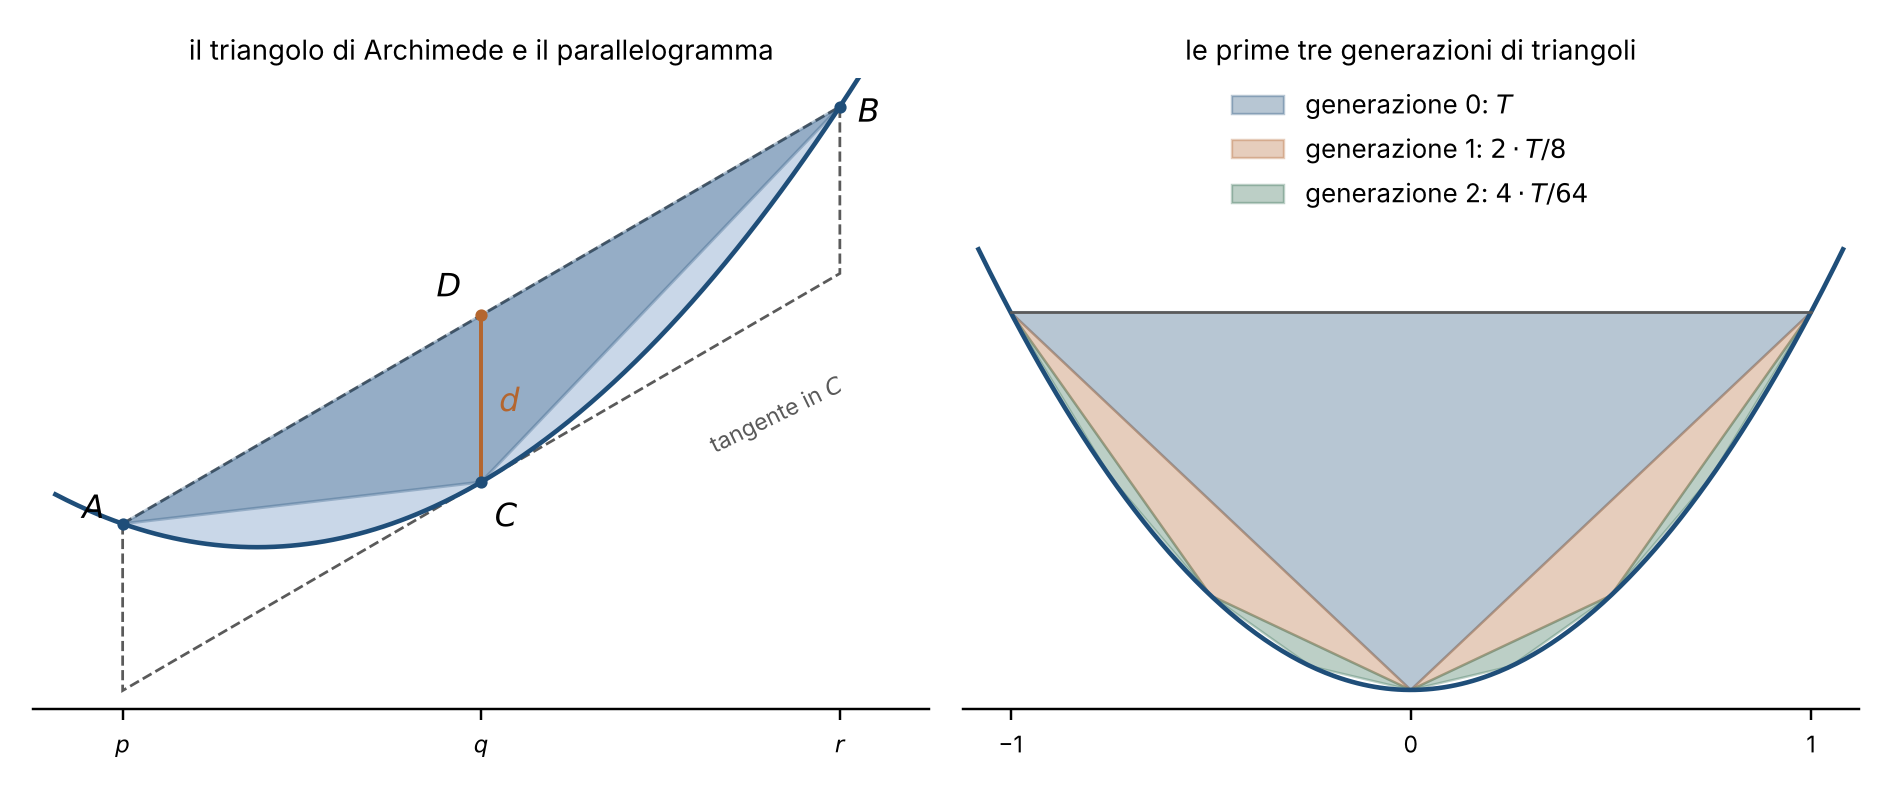
\includegraphics[width=\textwidth]{figure/archimede_parabola.png}
\caption{A sinistra, il segmento parabolico $\Sigma(p,r)$ (azzurro chiaro), il suo
triangolo di Archimede $ABC$ e il parallelogramma tratteggiato del
\cref{lem:triangolo-archimede}, delimitato dalla corda e dalla tangente in $C$, che
contiene il segmento e ha area doppia di quella del triangolo. A destra, i triangoli
delle prime tre generazioni per la corda di estremi $(\pm1,1)$: ogni generazione ha
area totale pari a $\frac14$ della precedente
(\texttt{python/fig\_archimede\_parabola.py}).}
\label{fig:archimede-parabola}
\end{figure}

\needspace{10\baselineskip}
Il segmento $\Sigma(p,r)$ si scompone nel triangolo $ABC$ e nei due segmenti
$\Sigma(p,q)$ e $\Sigma(q,r)$, di corde $AC$ e $CB$, senza punti interni comuni: per
$p\le x\le q$, ad esempio, la corda $AC$ divide il segmento verticale di $\Sigma(p,r)$
sopra $x$ in una parte che sta in $\Sigma(p,q)$ e una che sta nel triangolo. I due nuovi
segmenti hanno corde di larghezza $\frac w2$ e, per il lemma, triangoli di Archimede di
area $\frac18\cdot\frac{w^{3}}8$ ciascuno: insieme, un quarto del primo triangolo. È il
motore della dimostrazione.

\begin{proposizione}[Quadratura della parabola]\label{prop:quadratura-archimede}
Siano $p<r$ e sia $T=\frac{(r-p)^{3}}8$ l'area del triangolo di Archimede del segmento
parabolico $\Sigma(p,r)$. Se il segmento ha un'area, essa vale
\begin{equation}\label{eq:quadratura-archimede}
  \text{area }\Sigma(p,r)=\frac43\,T=\frac{(r-p)^{3}}6 .
\end{equation}
\end{proposizione}

\begin{schema}
\Ipotesi{$p<r$; \ l'area gode delle proprietà intuitive (aree elementari, additività,
confronto per inclusione).}
\Tesi{area $\Sigma(p,r)=\frac43\,T$, \ dove $T=\frac{(r-p)^{3}}8$ è l'area del
triangolo di Archimede.}
\end{schema}

\begin{strategia}
Si inscrivono nel segmento triangoli di generazioni successive: ogni generazione ha
area totale $\frac14$ della precedente, e l'unione delle prime $n+1$ generazioni è un
poligono la cui area è una somma geometrica finita, minore di $\frac43T$ per
$\frac T{3\cdot4^{n}}$. Ciò che resta scoperto è formato da segmenti più piccoli, e per
il \cref{lem:triangolo-archimede}(c) ha area al più doppia di quella della generazione
successiva. Archimede conclude con una \emph{doppia riduzione all'assurdo}: l'area del
segmento non può essere né maggiore né minore di $\frac43T$.
\end{strategia}

\begin{dimostrazione}
Sia $w=r-p$. Per $k\ge0$ intero, i punti $x_{j}=p+j\frac w{2^{k}}$,
$j=0,\dots,2^{k}$, dividono $[p,r]$ in $2^{k}$ parti uguali; chiamiamo \emph{segmenti di
generazione $k$} i $2^{k}$ segmenti parabolici $\Sigma(x_{j-1},x_{j})$, di corde di
larghezza $\frac w{2^{k}}$. Per il \cref{lem:triangolo-archimede}(b), ciascuno di essi
ha un triangolo di Archimede di area $\frac18\bigl(\frac w{2^{k}}\bigr)^{3}=\frac
T{8^{k}}$, e i triangoli di generazione $k$ hanno area totale
$2^{k}\cdot\frac T{8^{k}}=\frac T{4^{k}}$. Per la scomposizione descritta prima
dell'enunciato, ogni segmento di generazione $k$ è l'unione del suo triangolo e di due
segmenti di generazione $k+1$, senza punti interni comuni. Ripetendo la scomposizione,
per ogni $n\in\N$ il segmento $\Sigma(p,r)$ è l'unione del poligono $P_{n}$, formato dai
triangoli delle generazioni $0,1,\dots,n$, e dei $2^{n+1}$ segmenti di generazione
$n+1$, senza punti interni comuni.

\emph{L'area del poligono.} Per l'additività e per la somma della progressione
geometrica (\cref{prop:geometrica}) con $x=\frac14$,
\begin{equation}\label{eq:poligono-archimede}
  \text{area }P_{n}=T\Bigl(1+\frac14+\dots+\frac1{4^{n}}\Bigr)
  =T\,\frac{1-\frac1{4^{n+1}}}{1-\frac14}=\frac43\,T-\frac T{3\cdot4^{n}} .
\end{equation}

\emph{Ciò che resta scoperto.} Per il \cref{lem:triangolo-archimede}(c) e il confronto
per inclusione, ogni segmento di generazione $n+1$ ha area minore o uguale del doppio
del suo triangolo, cioè di $\frac{2T}{8^{n+1}}$. Sommando sui $2^{n+1}$ segmenti, la parte
scoperta $R_{n}=\text{area }\Sigma(p,r)-\text{area }P_{n}$ verifica
\begin{equation}\label{eq:resto-archimede}
  R_{n}\le2^{n+1}\cdot\frac{2T}{8^{n+1}}=\frac{2T}{4^{n+1}}=\frac T{2\cdot4^{n}} .
\end{equation}

\emph{La doppia riduzione all'assurdo.} Poniamo $\mathcal A=\text{area }\Sigma(p,r)$ e
$K=\frac43T$. Osserviamo che $4^{n}=(1+3)^{n}\ge1+3n>n$ per la disuguaglianza di
Bernoulli (\cref{teo:bernoulli}). Se fosse $\mathcal A>K$, per la proprietà di
Archimede (\cref{teo:archimede}) esisterebbe $n\in\N$ con $n>\frac T{2(\mathcal A-K)}$;
per la \eqref{eq:resto-archimede} si avrebbe $R_{n}\le\frac T{2\cdot4^{n}}<\frac T{2n}
<\mathcal A-K$, cioè $\text{area }P_{n}=\mathcal A-R_{n}>K$, contro la
\eqref{eq:poligono-archimede}, che dà $\text{area }P_{n}<K$. Se fosse $\mathcal A<K$,
esisterebbe $n\in\N$ con $n>\frac T{3(K-\mathcal A)}$, e per la
\eqref{eq:poligono-archimede} $K-\text{area }P_{n}=\frac T{3\cdot4^{n}}<\frac T{3n}<
K-\mathcal A$, cioè $\text{area }P_{n}>\mathcal A$: impossibile, perché il poligono $P_{n}$
è contenuto nel segmento. Esclusi i due casi, resta $\mathcal A=K=\frac43T$, e
$\frac43\cdot\frac{(r-p)^{3}}8=\frac{(r-p)^{3}}6$.
\end{dimostrazione}

\begin{osservazione}[La somma di Archimede e la serie geometrica]
\label{oss:somma-archimede}
Archimede ottenne la \eqref{eq:poligono-archimede} con una somma telescopica: ogni
termine, aumentato di un suo terzo, è un terzo del precedente,
$\frac1{4^{k}}+\frac13\cdot\frac1{4^{k}}=\frac13\cdot\frac1{4^{k-1}}$, e sommando per
$k=1,\dots,n$ si ha $1+\frac14+\dots+\frac1{4^{n}}+\frac13\cdot\frac1{4^{n}}=\frac43$.
Nel linguaggio del \cref{cap:serie}, la serie geometrica $1+\frac14+\frac1{16}+\cdots$
ha somma $\frac43$: la doppia riduzione all'assurdo fa le veci del passaggio al limite.
\end{osservazione}

\begin{esempio}[Due verifiche con il settore di parabola]\label{es:archimede-settore}
Per la corda di estremi $(\pm b,b^{2})$ la \eqref{eq:quadratura-archimede} dà
$\frac{(2b)^{3}}6=\frac43b^{3}$; con la \eqref{eq:area-parabola}, il segmento è il
rettangolo $[-b,b]\times[0,b^{2}]$ privato di due regioni congruenti al settore
\eqref{eq:settore-parabola}, e ha area $2b^{3}-2\cdot\frac{b^{3}}3=\frac43b^{3}$. Per la
corda di estremi $(0,0)$ e $(b,b^{2})$ si ottiene $\frac{b^{3}}6$, e infatti togliendo
il settore $S$ dal triangolo di vertici $(0,0)$, $(b,0)$, $(b,b^{2})$ resta
$\frac{b^{3}}2-\frac{b^{3}}3=\frac{b^{3}}6$. I triangoli di Archimede e i rettangoli
delle somme integrali portano allo stesso risultato.
\end{esempio}

\begin{notastorica}[Il \emph{Metodo} di Archimede]
La \emph{Quadratura della parabola}, indirizzata all'astronomo Dositeo di Pelusio,
contiene due dimostrazioni del teorema dei $\frac43$: una «meccanica», che equilibra il
segmento con un triangolo su una bilancia ideale, e quella con i triangoli inscritti che
abbiamo appena seguito. Entrambe, però, presuppongono di conoscere il risultato:
l'esaustione è un metodo di dimostrazione, non di scoperta, e già nel Seicento si
sospettava che Archimede possedesse un procedimento segreto per trovare i suoi teoremi.
La risposta arrivò nel 1906, quando il filologo danese Johan Ludvig Heiberg riconobbe, in
un libro di preghiere conservato a Costantinopoli, il testo raschiato di un codice di
opere di Archimede copiato nel \textsc{x} secolo, la cui pergamena era stata riutilizzata
nel 1229. Vi si trovava, in copia unica, il \emph{Metodo sui teoremi meccanici}, una
lettera a Eratostene in cui Archimede racconta di aver scoperto i suoi risultati
scomponendo le figure in infinite strisce parallele e bilanciandole su una leva, e
avverte che questo modo di ragionare suggerisce la verità ma non la dimostra. Il primo
esempio della lettera è proprio il segmento di parabola. Rimasto a lungo irreperibile,
il palinsesto ricomparve a un'asta nel 1998 ed è stato poi studiato a Baltimora con
tecniche di imaging multispettrale, che hanno restituito passi che Heiberg non era
riuscito a leggere. Le strisce del \emph{Metodo} sono le antenate degli indivisibili di
Cavalieri e dei rettangoli delle nostre somme integrali.
\end{notastorica}
